\chapter{Results and Discussion}\label{chap:Results}

\section{Performance Evaluation Metrics}

This section outlines the performance metrics used to evaluate the proposed framework. This evaluation is designed to verify that the proposed model gives a result that is better than the base model and other existing sudoku solvers. The mentioned performance indicators are the following:

\subsection*{Success Rate (SR)}
        \begin{equation}
        SR = \left( \frac{N_{success}}{N_{total}} \right) \times 100\%
        \end{equation}
        where $N_{total}$ is 100 unique general puzzles. A higher Success Rate means the solver is able to solve more sudoku puzzles thus better at searching the search space for a solution.    

\subsection*{Mean Time to Solution (MTTS)}
        The average time to generate a solution is an essential performance metric to determine the computational efficiency of the solver. 
        \begin{equation}
        MTTS = \frac{1}{N_{success}} \sum_{i=1}^{N_{success}} T_i
        \end{equation}
        where $T_i$ is the runtime of the $i$-th successful trial. 

\subsection*{Standard Deviation (Std)}
        As the ACO is stochastic, it may solve the puzzles in different runtime. This metric is used to determine how stable the solver is. 
        \begin{equation}
        Std = \sqrt{\frac{1}{N_{success}} \sum_{i=1}^{N_{success}} (T_i - MTTS)^2}
        \end{equation}
        A lower Standard Deviation show that the solver is able to solve the puzzle in similar timeframe. 

\subsection*{Iterations to Solve}

        This metric is used to count the number of iterations the solver took to generate a valid solution($f_{best} = \text{Total Cells}$). A lower value of this metric shows that the solver has the best balance between exploration and exploitation. 

\section{Implementation Details}

\begin{table}[H]
    \caption{Machine specifications}
    \centering
    \renewcommand{\arraystretch}{1.2} 
    \setlength{\tabcolsep}{10pt} 
    \begin{tabular}{|l|l|}
    \hline
    \textbf{Component}          & \textbf{Specification}                                \\ \hline
    Processor                   & AMD Ryzen 5 7530U (6 Cores, 12 Threads) @ 2.00 GHz    \\ \hline
    RAM                         & 16.0 GB                                               \\ \hline
    \end{tabular}
    \label{tab:machine_specifications}
\end{table}

As shown in Table~\ref{tab:machine_specifications}, the multi-threaded multi-colony ACO was implemented on a machine that is equipped with an AMD Ryzen 5 7530U processor which contains 6 physical cores and 12 threads. SudoSLVRR was able to execute the experiments as the machine is supported with 12 logical processors that allows the concurrent execution of multiple threads. The implementation of the solver is written in C++ which is known for its performance when it comes to multithreading capabilities. 

\section{Experimental Setups}
The experimental setup contains different sequence of experiments targeting specific objectives of this study. 


\subsection{Experiment 1: Ablation Study}
        This experiment evaluates the impact of individual parameters to the model's performance. This experiment addresses the second objective of this study allowing the proposed model to be fine-tuned. 

\subsection{Experiment 2: Single-Thread Multi-Colony ACO vs Multithread Multi-Colony ACO} 
	This experiment compares the performance of between single thread and multithread solvers. This highlights the impact of parallelization on the solver’s performance when solving sudoku puzzles. It is important to note that parallelization in this experiment involves collaboration with other threads. 

\subsection{Experiment 3: Without Thread Communication vs With Thread Communication}
        This experiment evaluates the necessity of information exchange between parallel threads. This, also, compares the performance of parallel independent runs against topology-aware and communicating threads. Communication topologies used in this experiment are ring and random communication topologies. 

\subsection{Experiment 4: Multithreaded Multi-Colony ACO vs State-of-the-Art Sudoku Solver}
        This experiment compares the performance of the proposed multithreaded multi-colony ACO solver against state-of-the-art sudoku solvers. This shows the robustness of the solver especially for high-order sudoku puzzle like $25 \times 25$.  

\subsection{Experiment 5: Model Deployment}
	This experiment addresses the last objective of this study which is to deploy the proposed solver as a functional web-based application. The deployment was implemented using Python Flask framework to manage both backend and frontend services and C++ for the implementation of the proposed solver. 
	The user of the web-based application should be able to choose a puzzle instance from a predefined list, create their own, or upload a text file given that it follows a specific format. Furthermore, the user should be able to adjust parameters before solving the puzzle. The application solves the inputted puzzle and displays the output puzzle in the interface as shown in Figure~\ref{web-app}.  

        \begin{figure}[H]
                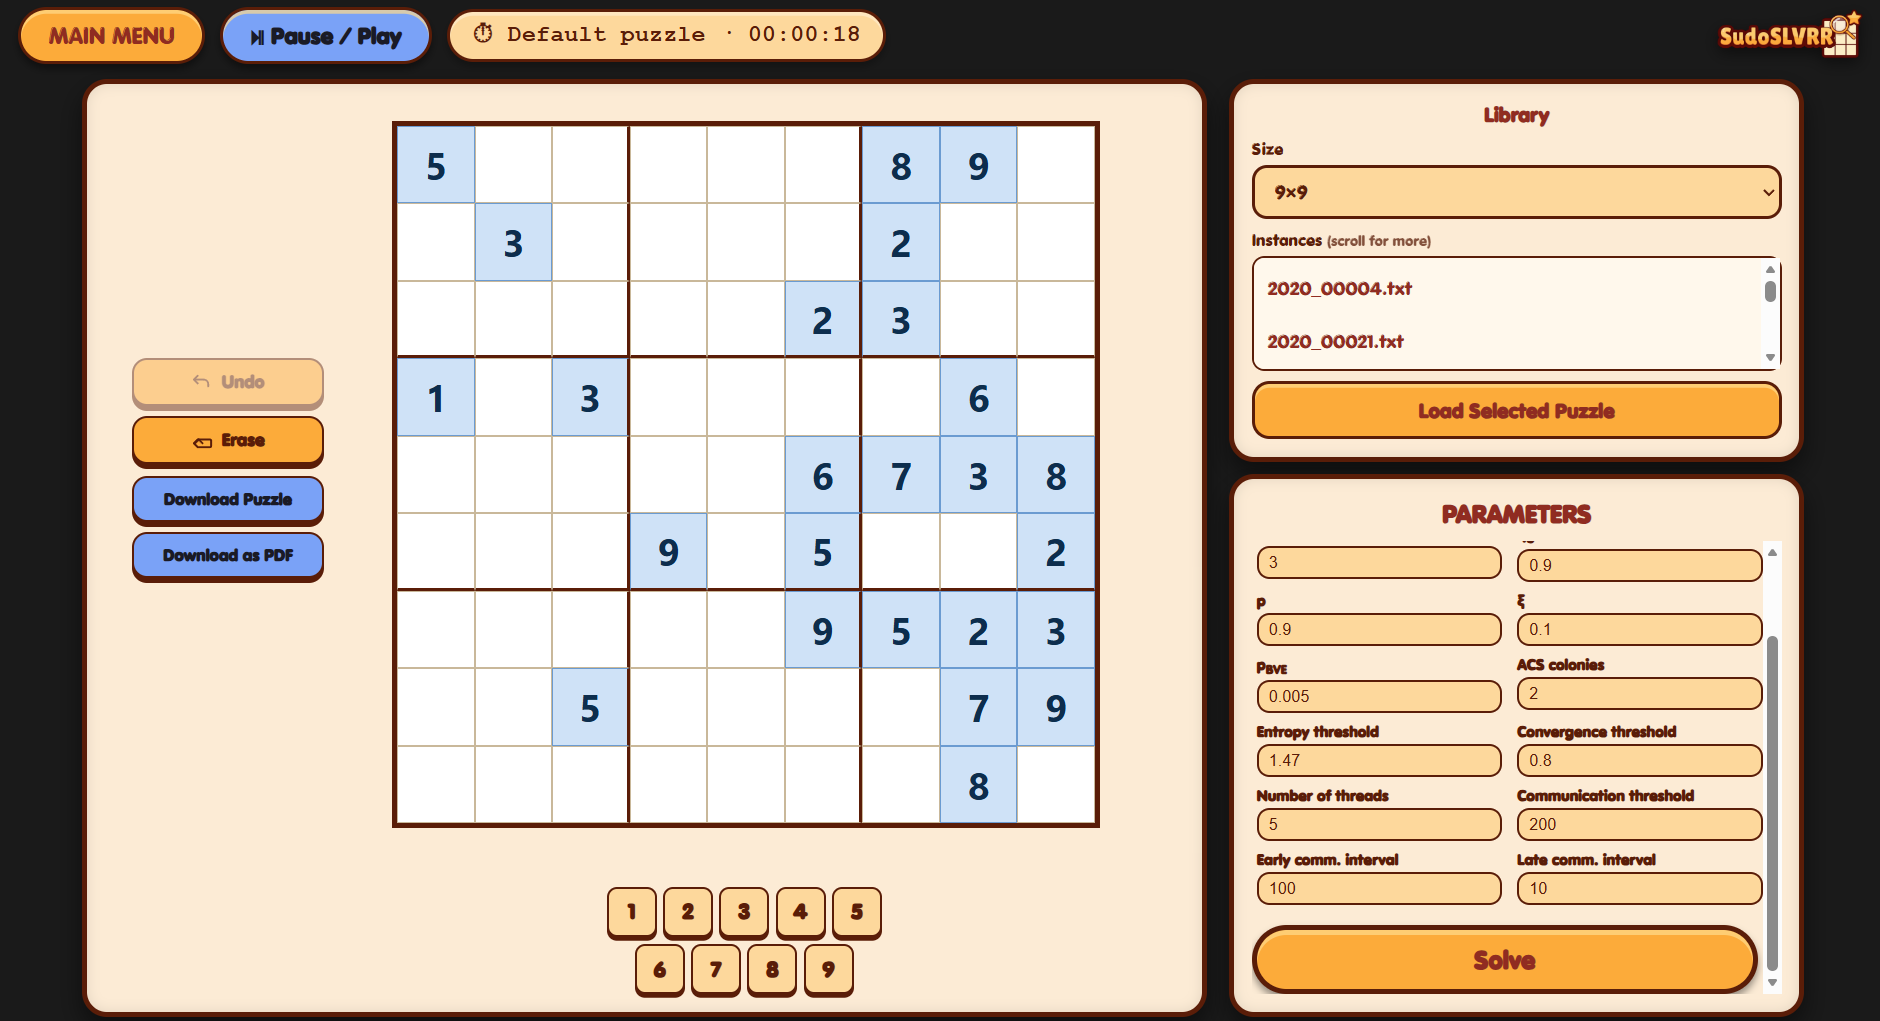
\includegraphics[width=\linewidth]{../figures/SudoSLVRR_Web.png} 
                \captionof{figure}{SudoSLVRR web-based application} 
                \label{web-app} 
        \end{figure}

\section{Results and Discussion}
\subsection{Experiment 1: Ablation Study}
        The final configuration for the proposed model, Multithread Multi-colony ACO Solver, was obtained through a series of experiment. Five different values for each 13 parameters are tried and observed its impact to the solver's perfomance. This was done by adjusting only one parameter at a time while holding other parameters constant at their baseline configuration (See Table~\ref{tab:baseline_parameters}). This experiment gave the best value for each parameter allowing the solver to maximize its potential in navigating a very complex solution space, especially of a large-scale $25 \times 25$ Sudoku. Table~\ref{tab:best_parameters} shows the summary of the best configuration of parameters for the proposed model. 
        \begin{table}[H]
                \caption{Best Configuration of Multithread Multi-colony ACO}
                \centering
                \renewcommand{\arraystretch}{1.2} 
                \setlength{\tabcolsep}{10pt} 
                \begin{tabular}{|l|l|}
                \hline
                \textbf{Parameter}                          & \textbf{Baseline Value}                               \\ \hline
                $q_0$ (Exploitation Factor)                 & 0.9                                        \\ \hline
                $\xi$ (Local Pheromone Update)              & 0.1                                         \\ \hline
                $\rho_0$ (Pheromone Persistence)            & 0.99                                        \\ \hline
                $\rho_{BVE}$ (Best Pheromone Evaporation)   & 0.0125                                                                            \\ \hline
                Number of ACS colonies                      & 6                                          \\ \hline
                Number of Ants (Per Colony)                 & 3                                           \\ \hline
                Entropy Threshold                           & 87.875\% of the Max Entropy (1.39)                              \\ \hline
                Convergence Threshold                     & 0.4                                                      \\ \hline
                Thread Count                                & 5                                         \\ \hline
                Communication Threshold                     & 200 iterations                             \\ \hline
                Early Communication Interval                & 120 iterations                           \\ \hline
                Late Communication Interval                 & 5 iterations                              \\ \hline
                \textbf{Timeouts}                           &                                                       \\ \hline
                $9 \times 9$ Sudoku                         & 9 seconds                                             \\ \hline
                $16 \times 16$ Sudoku                       & 30 seconds                                            \\ \hline
                $25 \times 25$ Sudoku                       & 180 seconds \\ \hline
                \end{tabular}
                \label{tab:best_parameters}
                \end{table}
        Tables~\ref{tab:ablation_coreACO_summary},~\ref{tab:ablation_timeout},~\ref{tab:ablation_multiColony}, and~\ref{tab:ablation_multithread} show the detailed results from the conducted ablation study. This contains the results of each parameter value accross three different puzzle sizes. 

\subsection{Experiment 2: Single-Thread Multi-Colony ACO vs Multithread Multi-Colony ACO} 
        This experiment shows the difference of the performance of single-thread multi-colony ACO and multithread multi-colony ACO. Furthermore, conducting this experiment shows the advantage of using concurrent exploration when solving combinatorial search space. 
        Table~\ref{tab:single_vs_multi_comparison} shows the results of running the single-thread multi-colony ACO (CP-DCM-ACO) and the multithread multi-colony ACO (MT-CP-DCM-ACO). The solvers processed the same set of instances consisting of 100 puzzles each grid size ($9\times9$, $16\times16$, and $25\times25$) 5 times. We can see from the table that multithreading does not improves the speed of the solver but also offers greater scalability. It is clear that by leveraging parallel processing, the solver can guarantee finding a solution even in extreme solution space. 

\begin{table}[H]
    \centering
    \caption{Performance Comparison of CP-DCM-ACO vs. MT-CP-DCM-ACO across $9 \times 9$, $16 \times 16$, and $25 \times 25$ Sudoku Instances (100 Puzzles, 5 Trial Runs).}
    \label{tab:single_vs_multi_comparison}
    \footnotesize
    \begin{tabular}{@{}llccc@{}}
        \toprule
        \textbf{Solver} & \textbf{Metric} & \textbf{Best} & \textbf{Worst} & \textbf{Average} \\
        
        % --- 9x9 Section ---
        \midrule
        \multicolumn{5}{c}{\textbf{9 $\times$ 9 Sudoku}} \\
        \midrule
        \multirow{3}{*}{\textbf{CP-DCM-ACO}} & Success Rate (\%) & 100 & 100 & 100 \\
                                             & Time (s) & $0.0667 \pm 0.0683$ & $0.1037 \pm 0.1064$ & $0.0830 \pm 0.0835$ \\
                                             & Iteration & 39.54 & 61.98 & 50.07 \\
        \cmidrule(lr){1-5}
        \multirow{3}{*}{\textbf{MT-CP-DCM-ACO}} & Success Rate (\%) & 100 & 100 & 100 \\
                                                & Time (s) & \boldmath{$0.0279 \pm 0.0258$} & \boldmath{$0.0315 \pm 0.0304$} & \boldmath{$0.0295 \pm 0.0290$} \\
                                                & Iteration & \textbf{11.23} & \textbf{12.29} & \textbf{11.68} \\
        
        % --- 16x16 Section ---
        \midrule
        \multicolumn{5}{c}{\textbf{16 $\times$ 16 Sudoku}} \\
        \midrule
        \multirow{3}{*}{\textbf{CP-DCM-ACO}} & Success Rate (\%) & 100 & 100 & 100 \\
                                             & Time (s) & $0.0549 \pm 0.0900$ & $0.1294 \pm 0.3873$ & $0.0835 \pm 0.1928$ \\
                                             & Iteration & 6.23 & 14.48 & 9.33 \\
        \cmidrule(lr){1-5}
        \multirow{3}{*}{\textbf{MT-CP-DCM-ACO}} & Success Rate (\%) & 100 & 100 & 100 \\
                                                & Time (s) & \boldmath{$0.0397 \pm 0.0230$} & \boldmath{$0.0535 \pm 0.1346$} & \boldmath{$0.0459 \pm 0.0617$} \\
                                                & Iteration & \textbf{3.03} & \textbf{3.93} & \textbf{3.46} \\
        
        % --- 25x25 Section ---
        \midrule
        \multicolumn{5}{c}{\textbf{25 $\times$ 25 Sudoku}} \\
        \midrule
        \multirow{3}{*}{\textbf{CP-DCM-ACO}} & Success Rate (\%) & 100 & 98 & 99 \\
                                             & Time (s) & $5.3496 \pm 6.5340$ & $7.5980 \pm 18.7057$ & $6.3411 \pm 10.4774$ \\
                                             & Iteration & 124.67 & 178.43 & 149.13 \\
        \cmidrule(lr){1-5}
        \multirow{3}{*}{\textbf{MT-CP-DCM-ACO}} & Success Rate (\%) & 100 & \textbf{100} & \textbf{100} \\
                                                & Time (s) & \boldmath{$3.9575 \pm 5.4078$} & $6.1483 \pm 10.0960$ & $5.4813 \pm 7.4532$ \\
                                                & Iteration & \textbf{42.29} & 53.17 & 49.24 \\
        \bottomrule
    \end{tabular}
\end{table}

\begin{figure}[H]
    \centering
    % --- Graph 1: Execution Time ---
    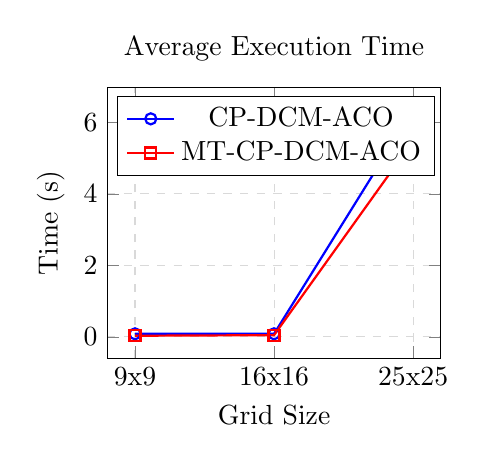
\begin{tikzpicture}
        \begin{axis}[
            width=0.48\textwidth,
            title={Average Execution Time},
            xlabel={Grid Size},
            ylabel={Time (s)},
            symbolic x coords={9x9, 16x16, 25x25},
            xtick=data,
            legend pos=north west,
            grid=major,
            grid style={dashed,gray!30},
        ]
            \addplot[color=blue, mark=o, thick] coordinates {(9x9,0.0830) (16x16,0.0835) (25x25,6.3411)};
            \addplot[color=red, mark=square, thick] coordinates {(9x9,0.0295) (16x16,0.0459) (25x25,5.4813)};
            \legend{CP-DCM-ACO, MT-CP-DCM-ACO}
        \end{axis}
    \end{tikzpicture}
    \hfill
    % --- Graph 2: Iteration Count ---
    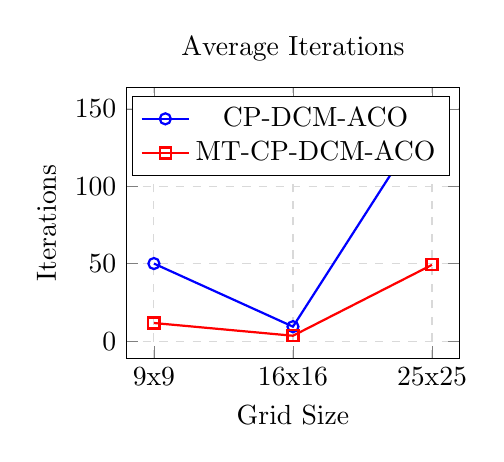
\begin{tikzpicture}
        \begin{axis}[
            width=0.48\textwidth,
            title={Average Iterations},
            xlabel={Grid Size},
            ylabel={Iterations},
            symbolic x coords={9x9, 16x16, 25x25},
            xtick=data,
            legend pos=north east,
            grid=major,
            grid style={dashed,gray!30},
        ]
            \addplot[color=blue, mark=o, thick] coordinates {(9x9,50.07) (16x16,9.33) (25x25,149.13)};
            \addplot[color=red, mark=square, thick] coordinates {(9x9,11.68) (16x16,3.46) (25x25,49.24)};
            \legend{CP-DCM-ACO, MT-CP-DCM-ACO}
        \end{axis}
    \end{tikzpicture}
    \caption{Shows the computational efficiency between CP-DCM-ACO and MT-CP-DCM-ACO across puzzle sizes.}
    \label{fig:performance_comparison}
\end{figure}

        Furthermore, Figure~\ref{fig:performance_comparison} shows that the computational costs of the MT-CP-DCM-ACO are still less than that of the CP-DCM-ACO even though additional overhead due to thread communication is introduced in the multithreaded solver. This result shows that multithread solver explores more regions of the solutions space thus speeding up the search for a solution. 

\subsection{Experiment 3: Without Thread Communication vs With Thread Communication}
        This experiment shows the necessity of the thread communication in searching a soluiton in a very complex solution space. Table~\ref{tab:with_vs_without_comm} shows that the setup that does not accomodate thread communication had less computational cost in $9\times9$ and $16\times16$ puzzles than with thread communication. It is because thread communication for this grid sizes is rarely triggered. The slight difference in computational cost betweeen the two setups are due to the initial overhead of the threads' communication. However when the grid sizes becomes larger like $25\times25$, colonies inside each threads requires more iterations to converge. Topology-aware setup allows the threads to exchange pheromone information thereby increasing the diversity of each thread. Uncommunicative setup suffers from stagnation as it get trapped to local optima thus failing to converge to a solution. 

\begin{table}[H]
    \centering
    \caption{Impact of Thread Communication on MT-CP-DCM-ACO across $9 \times 9$, $16 \times 16$, and $25 \times 25$ Sudoku Instances (100 Puzzles, 5 Trial Runs).}
    \label{tab:with_vs_without_comm}
    \footnotesize
    \begin{tabular}{@{}llccc@{}}
        \toprule
        \textbf{Solver Configuration} & \textbf{Metric} & \textbf{Best} & \textbf{Worst} & \textbf{Average} \\
        
        % --- 9x9 Section ---
        \midrule
        \multicolumn{5}{c}{\textbf{9 $\times$ 9 Sudoku}} \\
        \midrule
        \multirow{3}{*}{\textbf{Without Comm.}} & Success Rate (\%) & 100 & 100 & 100 \\
                                                & Time (s) & \boldmath{$0.0268 \pm 0.0208$} & $0.0360 \pm 0.0382$ & $0.0307 \pm 0.0291$ \\
                                                & Iteration & \textbf{10.30} & 13.57 & 11.75 \\
        \cmidrule(lr){1-5}
        \multirow{3}{*}{\textbf{With Comm.}}    & Success Rate (\%) & 100 & 100 & 100 \\
                                                & Time (s) & $0.0279 \pm 0.0258$ & \boldmath{$0.0315 \pm 0.0304$} & \boldmath{$0.0295 \pm 0.0290$} \\
                                                & Iteration & 11.23 & \textbf{12.29} & \textbf{11.68} \\
        
        % --- 16x16 Section ---
        \midrule
        \multicolumn{5}{c}{\textbf{16 $\times$ 16 Sudoku}} \\
        \midrule
        \multirow{3}{*}{\textbf{Without Comm.}} & Success Rate (\%) & 100 & 100 & 100 \\
                                                & Time (s) & $0.0426 \pm 0.0296$ & \boldmath{$0.0520 \pm 0.0630$} & $0.0481 \pm 0.0451$ \\
                                                & Iteration & $3.14$ & \textbf{3.57} & \textbf{3.37} \\
        \cmidrule(lr){1-5}
        \multirow{3}{*}{\textbf{With Comm.}}    & Success Rate (\%) & 100 & 100 & 100 \\
                                                & Time (s) & \boldmath{$0.0397 \pm 0.0230$} & $0.0535 \pm 0.1346$ & \boldmath{$0.0459 \pm 0.0617$} \\
                                                & Iteration & \textbf{3.03} & $3.93$ & $3.46$ \\
        
        % --- 25x25 Section ---
        \midrule
        \multicolumn{5}{c}{\textbf{25 $\times$ 25 Sudoku}} \\
        \midrule
        \multirow{3}{*}{\textbf{Without Comm.}} & Success Rate (\%) & 100 & 99 & 99.6 \\
                                                & Time (s) & \boldmath{$3.1261 \pm 3.32797$} & $2.9235\pm 3.3239$ & $3.1213 \pm 3.5223$ \\
                                                & Iteration & \textbf{41.80} & 49.11 & 45.46 \\
        \cmidrule(lr){1-5}
        \multirow{3}{*}{\textbf{With Comm.}}    & Success Rate (\%) & 100 & \textbf{100} & \textbf{100} \\
                                                & Time (s) & $3.9575 \pm 5.4078$ & $6.1483 \pm 10.0960$ & $5.4813 \pm 7.4532$ \\
                                                & Iteration & 42.29 & 53.17 & 49.24 \\
        \bottomrule
    \end{tabular}
\end{table}

\subsection{Experiment 4: Multithreaded Multi-Colony ACO vs State-of-the-Art Sudoku Solver}
        In table~\ref{tab:exp4_sota_comparison}, we can see that in all puzzle size the proposed model, MT-CP-DCM-ACO, outperforms all the other algorithms. For puzzle sizes $9\times9$ and $16\times16$, there is a clear reduction in execution times and number of iteration from the CP-ACS to CP-DCM-ACO, then to MT-CP-DCM-ACO. Then, it was magnified to $25\times25$ sudoku puzzle as baseline algorithms struggles to achieved a 100\% solution success rate. The multithreaded solver achieved 100\% success rate even in large-scale $25\times25$ sudoku because of its structured multi-level collaboration. 

        It is also clear in the table that multi-colony outperforms the single-colony solver across all grid sizes. The multi-colony solver already addresses the premature convergence of the single colony solvers by utilizing heterogeneous colonies that balances exploration and exploitation. By periodically triggering the collaboration between colonies, the improvement from the solver's performance can already be observed.
        
        However the multi-colony ACO, though enforces collaboration between heterogeneous ACS and MMAS colonies, still suffered from stagnation. This solver only covers few regions of a combinatorial search space when solving large-scale sudoku. By utilizing parallel processing and by placing the entropy-aware colonies inside each communicating threads, diversity increases thus overcoming premature convergence. The communication between threads also prevents redundant visits of the same region in the solution space. This is the reason why the multithread multi-colony ACO solver showed the best performance and results.
\begin{table}[H]
    \centering
    \caption{Performance Comparison of the State-of-the-Art (CP-ACS) vs. CP-DCM-ACO and MT-CP-DCM-ACO across $9 \times 9$, $16 \times 16$, and $25 \times 25$ Sudoku Instances (100 Puzzles, 5 Trial Runs).}
    \label{tab:exp4_sota_comparison}
    \footnotesize
    \begin{tabular}{@{}llccc@{}}
        \toprule
        \textbf{Solver} & \textbf{Metric} & \textbf{Best} & \textbf{Worst} & \textbf{Average} \\
        
        % --- 9x9 Section ---
        \midrule
        \multicolumn{5}{c}{\textbf{9 $\times$ 9 Sudoku}} \\
        \midrule
        \multirow{3}{*}{\textbf{CP-ACS}}     & Success Rate (\%) & 100 & 100 & 100 \\
                                             & Time (s) & $0.0852 \pm 0.0841$ & $0.1050 \pm 0.0988$ & $0.0945 \pm 0.0922$ \\
                                             & Iteration & 111.60 & 137.12 & 123.25 \\
        \cmidrule(lr){1-5}
        \multirow{3}{*}{\textbf{CP-DCM-ACO}} & Success Rate (\%) & 100 & 100 & 100 \\
                                             & Time (s) & $0.0667 \pm 0.0683$ & $0.1037 \pm 0.1064$ & $0.0830 \pm 0.0835$ \\
                                             & Iteration & 39.54 & 61.98 & 50.07 \\
        \cmidrule(lr){1-5}
        \multirow{3}{*}{\textbf{MT-CP-DCM-ACO}} & Success Rate (\%) & 100 & 100 & 100 \\
                                                & Time (s) & \boldmath{$0.0279 \pm 0.0258$} & \boldmath{$0.0315 \pm 0.0304$} & \boldmath{$0.0295 \pm 0.0290$} \\
                                                & Iteration & \textbf{11.23} & \textbf{12.29} & \textbf{11.68} \\
        
        % --- 16x16 Section ---
        \midrule
        \multicolumn{5}{c}{\textbf{16 $\times$ 16 Sudoku}} \\
        \midrule
        \multirow{3}{*}{\textbf{CP-ACS}}     & Success Rate (\%) & 96 & 93 & 94.2 \\
                                             & Time (s) & $0.3810 \pm 1.0603$ & $0.9794 \pm 2.8231$ & $0.7273 \pm 1.9593$ \\
                                             & Iteration & 61.12 & 166.41 & 120.71 \\
        \cmidrule(lr){1-5}
        \multirow{3}{*}{\textbf{CP-DCM-ACO}} & Success Rate (\%) & 100 & 100 & 100 \\
                                             & Time (s) & $0.0549 \pm 0.0900$ & $0.1294 \pm 0.3873$ & $0.0835 \pm 0.1928$ \\
                                             & Iteration & 6.23 & 14.48 & 9.33 \\
        \cmidrule(lr){1-5}
        \multirow{3}{*}{\textbf{MT-CP-DCM-ACO}} & Success Rate (\%) & 100 & 100 & 100 \\
                                                & Time (s) & \boldmath{$0.0397 \pm 0.0230$} & \boldmath{$0.0535 \pm 0.1346$} & \boldmath{$0.0459 \pm 0.0617$} \\
                                                & Iteration & \textbf{3.03} & \textbf{3.93} & \textbf{3.46} \\
        
        % --- 25x25 Section ---
        \midrule
        \multicolumn{5}{c}{\textbf{25 $\times$ 25 Sudoku}} \\
        \midrule
        \multirow{3}{*}{\textbf{CP-ACS}}     & Success Rate (\%) & 77 & 72 & 75 \\
                                             & Time (s) & $7.2533 \pm 12.3451$ & $12.8507 \pm 23.6261$ & $10.3381 \pm 18.5021$ \\
                                             & Iteration & 246.72 & 465.43 & 377.11 \\
        \cmidrule(lr){1-5}
        \multirow{3}{*}{\textbf{CP-DCM-ACO}} & Success Rate (\%) & 100 & 98 & 99 \\
                                             & Time (s) & $5.3496 \pm 6.5340$ & $7.5980 \pm 18.7057$ & $6.3411 \pm 10.4774$ \\
                                             & Iteration & 124.67 & 178.43 & 149.13 \\
        \cmidrule(lr){1-5}
        \multirow{3}{*}{\textbf{MT-CP-DCM-ACO}} & Success Rate (\%) & 100 & \textbf{100} & \textbf{100} \\
                                                & Time (s) & \boldmath{$3.9575 \pm 5.4078$} & $6.1483 \pm 10.0960$ & $5.4813 \pm 7.4532$ \\
                                                & Iteration & \textbf{42.29} & 53.17 & 49.24 \\
        \bottomrule
    \end{tabular}
\end{table}

\subsection{Experiment 5: Model Deployment}
        This experiment translates the multithread multi-colony ACO sudoku solver into a functional web-based application. Just like any sudoku game, user must follow the rules of sudoku in order to solve the puzzle. Upon accesing the application, user can choose either to play in experiment mode or game mode. 

        User can choose what values of the parameters he/she wants to try in experiment mode (See Figure~\ref{web-app:Experiment_Mode}). In game mode (See Figure~\ref{web-app:Game_Mode}), user can ask the application to solve the puzzle but automatically the multithread multi-colony ACO solver is called with its best configuration. User can see the real progress of the solver when it starts solving the puzzle because the application has a feature of real-time visualization of the puzzle. 

        \begin{figure}[H]
                \centering
                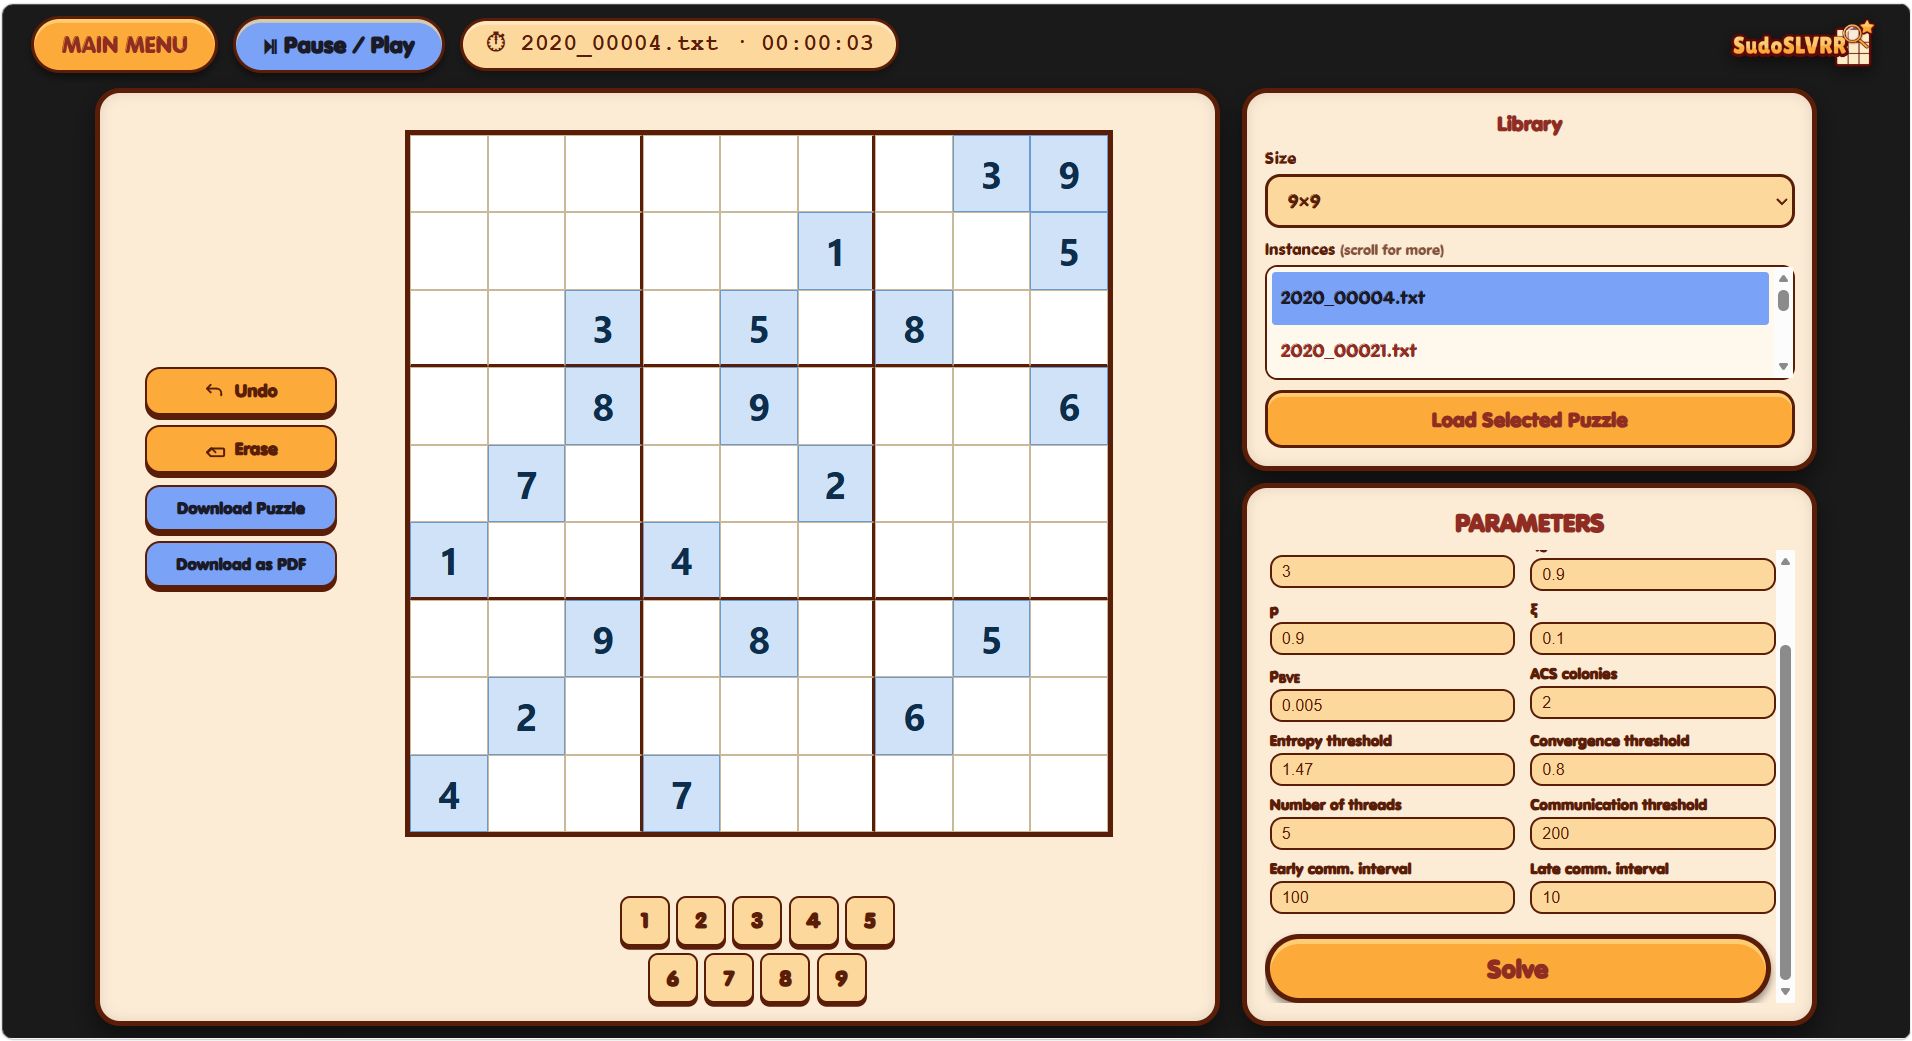
\includegraphics[width=0.5\linewidth]{../figures/Model_Deployment1_ForExperiment.png} 
                \captionof{figure}{SudoSLVRR web-based application: Experiment Mode} 
                \label{web-app:Experiment_Mode} 
        \end{figure}

        \begin{figure}[H]
                \centering
                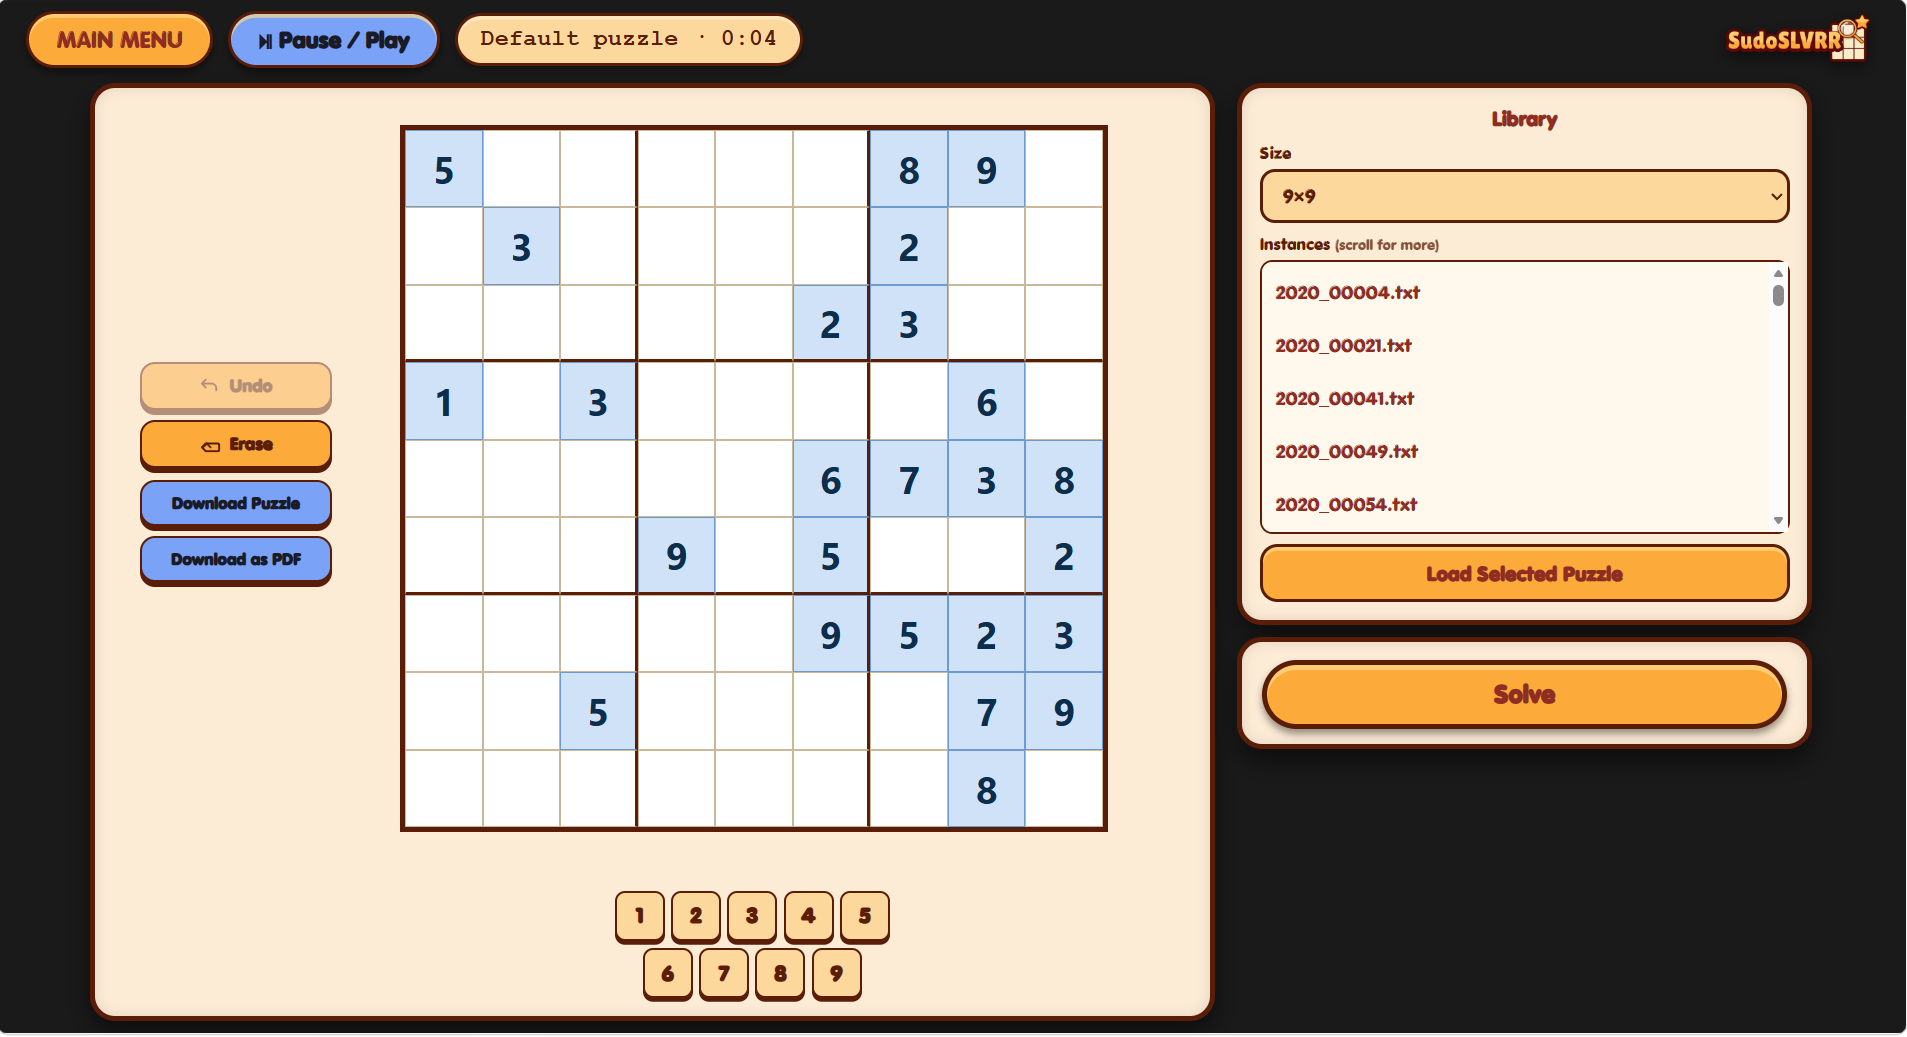
\includegraphics[width=0.5\linewidth]{../figures/Model_Deployment2_ForExperiment.png} 
                \captionof{figure}{SudoSLVRR web-based application: Game Mode} 
                \label{web-app:Game_Mode} 
        \end{figure}